\section{Introduction}
\label{sec:intro}
The Heavy Hitter problem refers to the objective of identifying the heaviest flows in a stream of data. In one variant of the problem, heavy flows are classified as those with a frequency above a threshold $t$. In this paper, we address a second variant of the problem--``top-$k$.'' In this variant, the heavy hitters are the top $k$ flows by frequency. 

There are many potential flows that can be analyzed in the context of the Heavy Hitters problem, including source IP addresses, destination IP addresses, transport port numbers, or five-tuples. Depending on the application of the algorithm, a different conception of flow may be appropriate. In this case, we employ our Heavy Hitters algorithm for DoS detection by identifying hosts that are responsible for sending the most traffic through an ISP link. Due to the nature of Internet traffic, a relatively few number of hosts are responsible for sending the majority of packets through a network. In fact, the top 3 percent of hosts may account for over half of the packets traveling through an ISP link in a given time period. Figure~\ref{fig:cumulative}, a graph of cumulative traffic addressed to/from the top $k$ sources/destinations, reveals two important conclusions about the distribution of traffic. First, there are approximately twice as many destinations as sources, and as a result, these sources account for more traffic on average. Second, for both source addresses and destination addresses, the heaviest hitters are responsible for a highly disproportionate amount of network traffic. Through the rest of this paper, we consider the frequency of packets identified by source IP address as our measure of heavy hitters.
\begin{figure}[t]
  \centering
    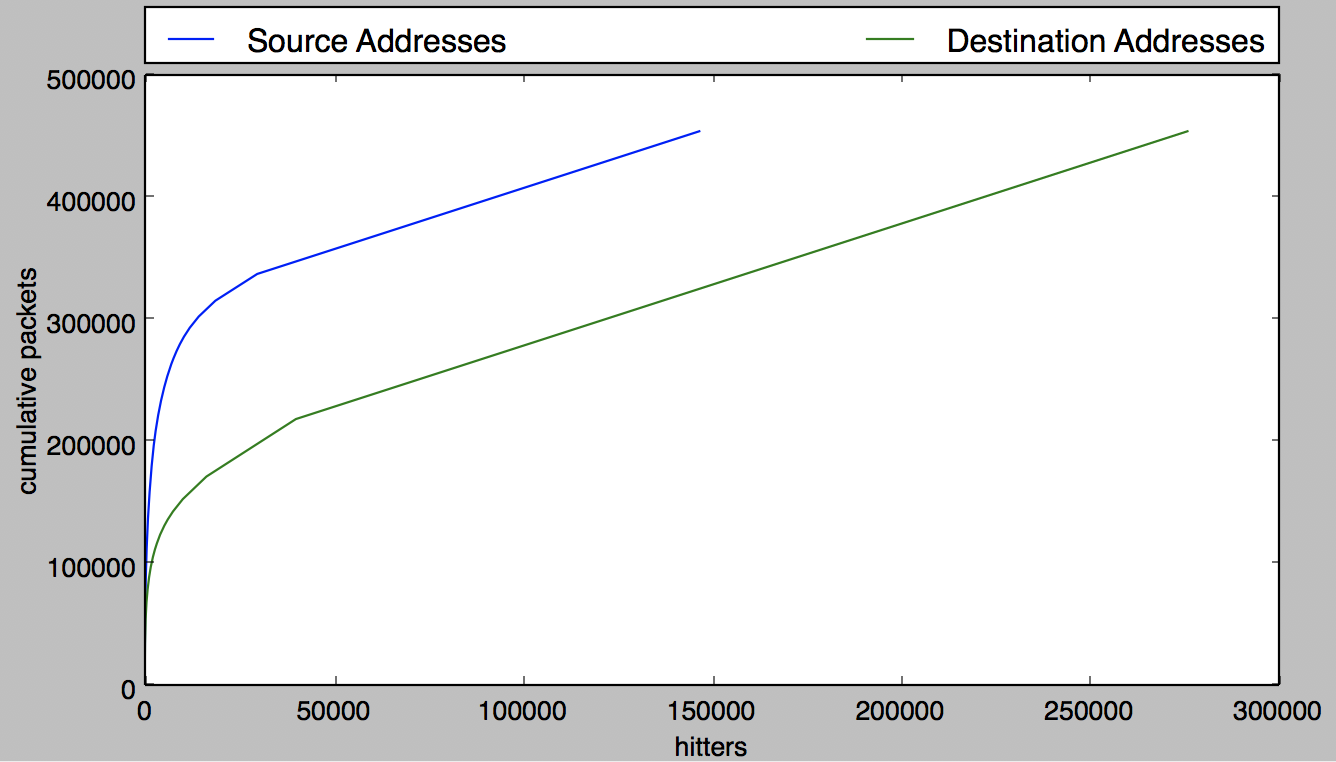
\includegraphics[scale=0.3]{cumulative}
     \caption{Graph of the cumulative traffic addressed to/from the top $k$ sources/destinations, captured from an ISP backbone link}
     \label{fig:cumulative}
\end{figure}